% вторая часть

\section{Описание предметной области}

\subsection{Android Studio}
Android Studio - полностью укомплектованная платформа для разработки и тестирования приложений под операционную систему Android. Разработчики этой оболочки (компания Google) внедрили весь необходимый инструментарий для удобного и качественного проектирования новых приложений и доработки существующих. Программа включает в себя такие компоненты как Android SDK, все версии операционки Android, эмулятор для запуска приложений, элементы тестирования и отладки программ.

Создавая новый проект, будет доступна полная структура приложения со всеми файлами, что позволяет более четко и продуманно организовать сам процесс разработки. Очень удобно реализован показ вносимых изменений и дополнений - визуально в реальном времени происходят преобразования в зависимости от заданных действий. Что немаловажно, программа позволяет делать разработку приложений для всех версий ОС Andriod и для различных устройств - можно предварительно оценить внешний вид программы, например, под планшет или смартфон.

Среда Android Studio предназначена как для небольших команд разработчиков мобильных приложений (даже в количестве одного человека), или же крупных международных организаций с GIT или другими подобными системами управления версиями. Опытные разработчики смогут выбрать инструменты, которые больше подходят для масштабных проектов. Решения для Android разрабатываются в Android Studio с использованием Java или C++. В основе рабочего процесса Android Studio заложен концепт непрерывной интеграции, позволяющий сразу же обнаруживать имеющиеся проблемы. Продолжительная проверка кода обеспечивает возможность эффективной обратной связи с разработчиками. Такая опция позволяет быстрее опубликовать версию мобильного приложения в Google Play App Store. В Android Studio есть удобная маркировка кода, которая позволит без труда ориентироваться в больших проектах. Кроме того, отдельные компоненты можно изменять простым перетаскиванием в другое нужное место, что значительно упрощает редактирование.

\subsection{Java}
Преимущества языка Java
\begin{itemize}
	\item Одно из основных преимуществ языка Java — независимость от платформы, на которой выполняются программы: один и тот же код можно запускать под управлением операционных систем Windows, Solaris, Linux, Machintosh и др. 
	Это действительно необходимо, когда программы загружаются через Интернет для последующего выполнения под управлением разных операционных систем.
	\item Другое преимущество заключается в том, что синтаксис языка Java похож на синтаксис языка C++, и программистам, знающим языки С и C++, его изучение не составляет труда.
	\item Кроме того, Java — полностью объектно-ориентированный язык, даже в большей степени, чем C++. Все сущности в языке Java являются объектами, за исключением немногих основных типов (primitive types), например чисел.
	\item Исключена возможность явного выделения и освобождения памяти.	Память в языке Java освобождается автоматически с помощью механизма сборки мусора. Программист гарантирован от ошибок, связанных с неправильным использованием памяти.
	\item Безопасный: методы проверки подлинности основаны на шифровании с открытым ключом.
	\item Динамический: программирование на Java считается более динамичным, чем на C или C++, так как он предназначен для адаптации к меняющимся условиям. Программы могут выполнять обширное количество во время обработки информации, которая может быть использована для проверки и разрешения доступа к объектам на время выполнения.
\end{itemize}

\subsection{Технические требования.}

Необходимая задача при реализации проекта - адаптация существующего метода преобразования 2D в 3D для использования под управлением операционной системы Android.

В ходе выполнения проекта будут созданы мобильные приложения со следующими характеристиками:

\begin{itemize}
	\item мобильное приложение, функционирующее под управлением операционной системы Android версии не ниже 5.0.
	\item специальных дополнительных требований к аппаратному обеспечению мобильных устройств не предъявляется. Они соответствуют требованиям, накладываемым вышеперечисленными версиями ОС.
	\item мобильные приложения должны функционировать на устройствах с разными размерами экрана от 2.6 до 6 дюймов с разрешениями от 240х320 до 1440х2560 пикселей.
	\item источник данных для конвертирования - файлы в формате jpeg из галереи мобильного устройства или фотография, сделанная штатной фотокамерой мобильного устройства.
	\item мобильные приложения должны обеспечивать конвертацию сделанных фотокамерой изображений при максимальном качестве съемки не менее 10 Мп.
	\item формат данных, в которых сохраняются результаты --- анаглиф файлы (формат jpeg), стерео пара (формат jps), анимированные файлы в формате gif.
	\item ориентировочное время преобразования 2D в 3D не должно превышать 5 секунд.
\end{itemize}

\subsection{Изучение основ разработки мобильного приложения в среде Android Studio}

Android основан на Linux. Между приложением и ядром лежит слой API и слой библиотек на нативном коде. Приложение выполняется на виртуальной машине Java (Dalvik Virtual Machine).
В Android можно запускать много приложений. Но одно из них есть главным и занимает экран. От текущего приложения можно перейти к предыдущему или запустить новое. Это похоже на браузер с историей просмотров.

Каждый экран пользовательского интерфейса представлен классом Activity в коде. Различные Activity содержатся в процессах. Activity может даже жить дольше процесса. Activity может быть приостановлена и запущена вновь с сохранением всей нужной информации.(рисунок~\ref{fig:activity})

\begin{figure}[H]
	\centering
	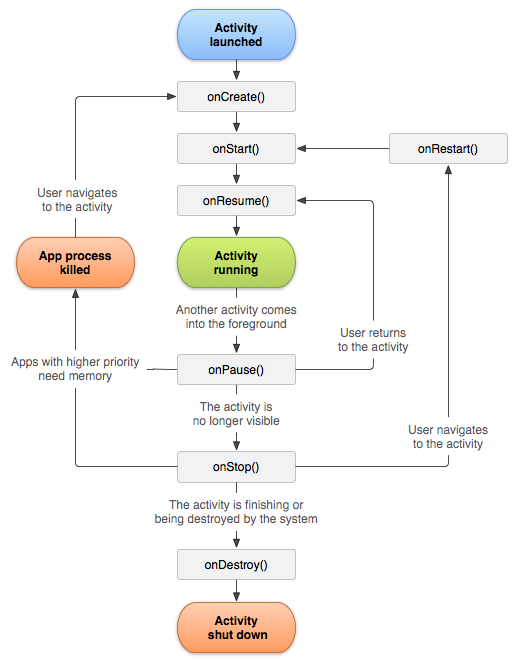
\includegraphics[width=0.6\linewidth]{pics/activity}
	\caption{activity}
	\label{fig:activity}
\end{figure}

Android использует специальный механизм описания действий основанный на Intent. Когда нужно выполнить действие (сделать звонок, послать письмо, показать окно), вызывается Intent.

Также Android содержит сервисы подобные демонам в Linux для выполнения нужных действий в фоновом режиме (например, проигрывание музыки).
Для обмена данными между приложениями используются Content providers (провайдеры содержимого).

Содержимое Activity формируется из различных компонентов, называемых View. Самые распространенные View - это кнопка, поле ввода, чекбокс и т.д. (рисунок~\ref{fig:view})

\begin{figure}[H]
	\centering
	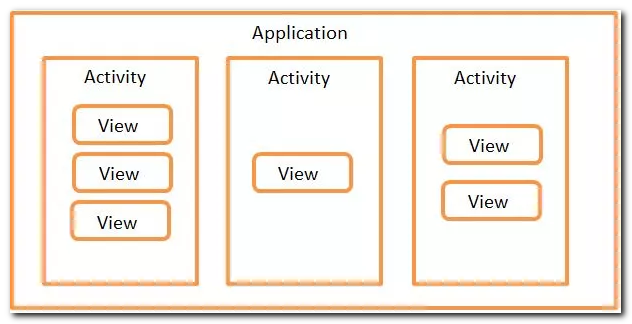
\includegraphics[width=0.6\linewidth]{pics/view}
	\caption{view}
	\label{fig:view}
\end{figure}

Необходимо заметить, что View обычно размещаются в ViewGroup. Самый распространенный пример ViewGroup – это Layout. Layout бывает различных типов и отвечает за то, как будут расположены его дочерние View на экране.

LinearLayout – отображает View-элементы в виде одной строки (если он Horizontal) или одного столбца (если он Vertical).

TableLayout – отображает элементы в виде таблицы, по строкам и столбцам.

RelativeLayout – для каждого элемента настраивается его положение относительно других элементов.

AbsoluteLayout – для каждого элемента указывается явная позиция на экране в системе координат (x,y)

\subsection{Основные компоненты пользовательского интерфейса мобильного приложения в Android}

В Android используется UI-фреймворк, сравнимый с другими полнофункциональными UI-фреймворками, применяемыми на локальных компьютерах. Он является более современным и асинхронным по природе. По существу, UI-фреймворк Android относится уже к четвертому поколению, если считать первым поколением традиционный прикладной интерфейс программирования Microsoft Windows, основанный на С, а MFC (Microsoft Foundation Classes, библиотека базовых классов Microsoft на основе C++) - вторым. В таком случае UI-фреймворк Swing, основанный на Java, будет третьим поколением, так как предлагаемые в нем возможности дизайна значительно превосходят по гибкости MFC. Android UI, JavaFX, Microsoft Silverlight и язык пользовательских интерфейсов Mozilla XML (XUL) относятся к новому типу UI-фреймворков четвертого поколения, в котором UI является декларативным и поддерживает независимую темизацию.

При программировании в пользовательском интерфейсе Android применяется объявление интерфейса в файлах XML. Затем эти определения представления (view definitions) XML загружаются в приложение с пользовательским интерфейсом как окна. Даже меню приложения загружаются из файлов XML. Экраны (окна) Android часто называются активностями (activities), которые включают в себя несколько видов, нужных пользователю, чтобы выполнить логический элемент процесса. Виды (views) являются основными элементами, из которых в Android состоит пользовательский интерфейс. Виды можно объединять в группы (view groups). Для внутренней организации видов используются давно известные в программировании концепции холст (canvas), рисование (painting) и взаимодействие пользователя с системой (user interaction).

Такие составные представления, в которые входят виды и группы видов, работают на базе специального логического заменяемого компонента пользовательского интерфейса Android.

Одной из ключевых концепций фреймворка Android является управление жизненным циклом (lifecycle) окон явлений (activity windows). В системе применяются протоколы, поэтому Android может управлять ситуацией по мере того, как пользователи скрывают, восстанавливают, останавливают и закрывают окна явлений.